\documentclass[a4paper, 12pt]{article}

\usepackage[utf8]{inputenc}
\usepackage{latexsym,amsfonts,amssymb,amsthm,amsmath}
\usepackage{setspace}
\usepackage{physics}
\usepackage{graphicx}
\usepackage{newtxtext}
\usepackage{extsizes}
\setlength{\parindent}{0in}
\setlength{\oddsidemargin}{0in}
\setlength{\textwidth}{6.5in}
\setlength{\textheight}{8.8in}
\setlength{\topmargin}{0in}
\setlength{\headheight}{8pt}

\onehalfspacing


\title{
  \vspace{-1.5cm}
  \textbf{Hypothesis testing}
  \vspace{-1.5cm}
}
\date{}

\begin{document}

\maketitle

\section{Introduction}
Point estimation and confidence interval estimation are important components of statistical analysis. But in many practical problems one has to decide whether to accept or reject a claim about a parameter or distribution. The procedure for deciding whether a hypothesis is correct or not is called \textbf{hypothesis testing}. This is one of the most widely used statistical inference tools\\

\textbf{Example:} We want to check if a coin is fair, i.e. does $p = 0.5$ in the binomial
distribution?

For this purpose, the coin is tossed n times and a sample of the obtained
outcomes is formed. Based on the obtained results, a statistical test
should be conducted in which it should be decided whether the
assumption (hypothesis) that the coin is fair will be accepted or rejected. \\



\textbf{Example :} The average waiting time of customers in one bank was 5 minutes.
We want to check if there has been a reduction in the average waiting
time since the new counter was introduced?

For this purpose, a certain number of customers are randomly selected and a sample of their waiting times is formed. Based on the obtained results, a statistical test should be conducted in which it should be decided whether the assumption (hypothesis) that the waiting time is reduced will be accepted or rejected.




\section{Statistical hypothesis}

\textbf{Definition 1.} Any assumption about the population, about the distribution of some of its features, about the values of some parameters of the feature, etc. it is called a \textbf{statistical hypothesis}.


The procedure by which, based on the data from a given sample, the correctness of the set hypothesis is checked is called a \textbf{statistical test}.

\subsection{Parametric and non-parametric hypotheses}

If the type (functional form) of the function $F(x,\theta)$ is known, and the parameters are unknown and some values are assumed for them, we say that the hypothesis is parametric, and in any other case we say that the hypothesis is non-parametric.

Examples:

\begin{itemize}
  \item  Let it be given that a random variable X has a normal distribution. Then the
  hypothesis "Mean of X is 0" is a parametric hypothesis and refers to $\mu$ in $N(\mu, \sigma^2)$
  \item Let X and Y be random variables with a normal distribution. Then the
  hypothesis "The variances of X and Y are equal" is a parametric hypothesis.
  \item  "The random variable X has a normal distribution" is a non-parametric
  hypothesis.
  \item  "The random variable X has a Poisson distribution $P(1)$" is a non-parametric
  hypothesis.
  \item  "Random variables X and Y are independent" is a non-parametric hypothesis.
\end{itemize}

As we can see from the previous two examples (with a faircoin and the expected waiting time at the bank), the testing procedure comes down to deciding on one of two mutually exclusive hypotheses.\\

More precisely, if one is accepted, the other is automatically rejected, and vice versa.\\

So in the first example, one hypothesis is that the coin is fair, or the probability of a head (and thus tails) is $1/2$, and the second hypothesis is that that probability is different than $1/2$.

In the second example, one hypothesis is that the waiting time will remain at 5 minutes, and the second is that the waiting time will decrease with the introduction of the new  counter.\\

The hypothesis being tested is called the \textbf{null hypothesis} and is denoted by $H_0$, and the opposite is called the \textbf{alternative hypothesis} and is denoted by $H_a$.\\


The null hypothesis is usually chosen based on some standards for the specific feature or the values that were current until the last measurement.\\


So, for the first example, if $p$ is the probability of a head, then

\[H_0: p=1/2\]
\[H_a: p\neq1/2\]

For the second example, if $\mu_1$ is the expected waiting time before the introduction of a new counter, and $\mu_2$ is the expected waiting time after the introduction of a new counter, then

\[H_0: \mu_1 = \mu_2\]
\[H_a: \mu_1 > \mu_2\]


\section{Parametric hypotheses}

In the further part of this lecture, we will focus on parametric hypothesis testing. The examples given on the previous slide are examples of parametric hypotheses.\\


Hypotheses in which only one value of the unknown parameter appears are called simple hypotheses. Thus, the hypothesis $H_0: p = 1/2$ is a \textbf{simple hypothesis}.\\


A hypothesis in which multiple values of the parameter are allowed for the parameter is called a \textbf{complex hypothesis}. The hypothesis $H_a: p = 1/2$ is a complex hypothesis, because here for $p$ all values from the interval $(0,1)$ that are different from $1/2$ are allowed.

\subsection{One-sided and two-sided test}

In the fair coin example, we made the following hypotheses:

\[H_0: p=1/2\]
\[H_a: p\neq1/2\]

Since the alternative hypothesis is  $H_a: p\neq1/2$ , such a test is called \textbf{two-sided test.} \\

In some cases, hypotheses can be tested as


\[H_0: p=1/2 \quad  H_0: p = 1/2 \]
\[H_a: p > 1/2 \quad  H_a: p<1/2\]

In that case, we say that the test is \textbf{one-sided}.\\

\section{Hypothesis testing}

The procedure that leads to deciding on a particular hypothesis is called hypothesis testing.\\

Hypothesis testing procedures rely on the use of information that can be obtained from a random sample taken from the population of interest.\\

If this information is consistent with the hypothesis, we will conclude that the hypothesis is correct. Conversely, if this information is inconsistent with the hypothesis, we will conclude that the hypothesis is incorrect.\\

It should be emphasized that the correctness of a hypothesis can never be known with certainty unless we can examine the entire population, which is impossible in most practical situations.\\

Therefore, hypothesis testing procedures are developed with a certain probability of reaching the wrong conclusion\\

\subsection{Type I and II error}

A false conclusion would be reached if we rejected the null hypothesis when it is true or if we accepted the null hypothesis when it is false (i.e. the alternative hypothesis is true). We therefore define two types of errors.


\textbf{Definition 2.} The error committed by rejecting the null hypothesis when it is true is called a \textbf{Type I error}. The error committed by accepting the null hypothesis when it is not true is called a \textbf{Type II error}.\\

Therefore, during any statistical hypothesis testing, four different situations are possible that determine whether the final solution is correct or incorrect. They are given in then table.

\begin{table}[h!]
\centering
\begin{tabular}{|l|l|l|}
\hline
\textit{}                      & $H_0$ is correct      & $H_0$ is not correct   \\ \hline
The test rejects $H_0$         & \textbf{Type I error} & No error               \\ \hline
The test does not reject $H_0$ & No error              & \textbf{Type II error} \\ \hline
\end{tabular}
\end{table}


Since our solution is based on random variables, we can define probabilities to Type I and Type II errors. We denote these probabilities by $\alpha$ and $\beta$, respectively, that is

\[ \alpha = P(\text{Type I error}) = P(H_0 \text{ is rejected} | H_0 \text{ is correct} ) \]
\[ \beta = P(\text{Type II error}) = P(H_0 \text{ is accepted} | H_0 \text{ is not correct} ) \]

The probability of a type I error is also called the significance
level of the test.

\subsection{Test power}

The quantity $1 - \beta$ is called the power of the test, and corresponds to the probability of rejecting the null hypothesis when it is not true.\\


The power of a test is actually a measure of the sensitivity of the test, where sensitivity is the ability of the test to detect differences.\\

We want the tests we are going to use to have as little type In error as possible and as little type II error as possible. However, there are no tests that simultaneously minimize the probabilities of both types of error.\\

Therefore, when testing hypotheses, the probability of a type I error or the significance level of the test is given in advance, and then tests are sought that have the smallest possible type II error, that is, the highest power.\\

\textbf{Example 1: } It is known that there are 10 balls in a box, but it is not certain whether there are 6 red and 4 green balls or 5 red and 5 green balls. Therefore, the following hypotheses are defined:
\[
H_0:\ \text{there are 6 red and 4 green balls in the box;}
\]
\[
H_a:\ \text{there are 5 red and 5 green balls in the box.}
\]

A ball is drawn from the box and the following test rule is defined:

The null hypothesis $H_0$ is not rejected if and only if a red ball is drawn; otherwise, $H_0$ is rejected.

Determine the probabilities of Type I and Type II errors.


\subsection{Choice of $\alpha$}
Most often, it is chosen $\alpha = 0.05$ or $\alpha = 0.01$.\\

$\alpha$ is the probability of rejecting the null hypothesis when it is
true. It shows the following:


Let the test be repeated several times.\\

We will consider each repetition of the test as an attempt to findn evidence that the null hypothesis is false.\\

If $\alpha = 0.05$ , then it can be considered that such evidence will be found in at most $5\%$ of trials, if the null hypothesis is true.\\

If, on the other hand,$\alpha = 0.01$, it means that when repeating the test several times, the null hypothesis will not be accepted in atn most $1\%$ of cases, if it is correct.\\


\section{Statistical test. Test statistics}

\textbf{Definition 3.} Any rule according to which at each realization $x$
of the random sample $X$ we either do not reject or reject the
hypothesis $H_0$ is called a \textbf{statistical test}.\\

We will base test rules or statistical tests on the values of certain statistics defined on the random sample which are called test statistics.\\


The next step in the null hypothesis testing procedure is the selection of the test statistic. That choice depends on then hypothesis we are testing.

\begin{itemize}
  \item One usually starts from a parameter estimator that has certain optimal
properties.
\item If hypotheses about the mean and the variance of the statistical feature are tested, it is usually started from the maximum likelihood estimator or from an estimator obtained by the method of moments.
\end{itemize}

\subsection{Critical domain}

The step before the last one in a statistical test is the determination of the \textbf{critical domain}.\\

It is, in fact, the area of rejection of the null hypothesis. The real axis is divided into two subareas: the area of acceptance of the null hypothesis and the area of its rejection (critical domain).\\

We will denote the critical domain by $C$ and it is chosen so that the probability that the test statistic (for example, $Z$) receives a value belonging to that critical domain, if the null hypothesis is true, is at most $\alpha$, i.e.

\[ P \{  Z \in C  | H_0 \text{ is correct}\} \leq \alpha\]

Note that the latter probability is, in fact, the probability of a Type I error, that is, the probability of rejecting the null hypothesis if it is true.\\

The critical domain $C$ is chosen such that the probability should be less than or equal to $\alpha$


\subsection{Most powerful critical domain}

As previously stated, one usually tries for a given probability of error of type I $\beta$, to determine the minimum value of the error of type II $\beta$.\\

The critical domain for which this is satisfied is called the optimal critical domain or \textbf{the most powerful critical domain}.\\

Hence, if $C^*$ is the most powerful critical domain, then for every other critical domain $C$ holds:

\[ P \{ Z \notin H_a \text{ is correct} \} \leq P \{ Z \notin C \text{ is correct} \}  \]


Thereby, the probability $P \{ Z \notin C \text{ is correct} \}$ is the probability of a type II error. Well, the last equality shows that the probability of a type II error is the smallest if we have the most powerful critical domain.\\

There are methods for determining the most powerful critical domain for testing a hypothesis, but we will not cover those methods here.\\

\section{Making a decision}

In the final step of the testing process, the value of a test statistic
based on a given sample is calculated and checked to see if it
belongs to the specified critical domain $C$.


\begin{itemize}
  
\item If that value belongs to $C$, then the null hypothesis is rejected as false,
otherwise
\item the null hypothesis is not rejected, i.e. is accepted as correct.


\end{itemize}


If the data from the random sample is such that $H_0$ is rejected we say that the difference between the data and the null hypothesis is significant or the test is significant.\\

If, according to the random sample, the null hypothesis $H_0$ is not rejected, we say that the data support the null hypothesis or the test is not significant

\section{Hypothesis testing algorithm}

\begin{itemize}
  \item [1.] From the context of the task identify the parameter of interest.
  \item [2.] Define the null hypothesis, $H_0$, and a corresponding alternative
  hypothesis, $H_a$
  \item [3.] The significance level of the test $\alpha$ is chosen.
  \item [4.] An appropriate test statistic is determined.
  \item [5.] The critical domain $C$ for the selected statistic is determined.
  \item [6.] The value of the test statistic is calculated.
  \item [7.] It is checked whether the calculated value of the test statistic
  belongs to the critical domain $C$ or not.
  \item [8.] If it does, then the null hypothesis is rejected as false, otherwise,
  it is accepted as true.
\end{itemize}


\newpage
\section{TESTS FOR ONE FEATURE}

\subsection{Tests for statistical mean of a feature}

Let $(X_1, \ldots, X_n)$ be a random sample of the variable $X$, whose mean is unknown.

We will consider tests for the mean of the variable $X$ in two cases:

\begin{itemize}
    \item The variable has a \textbf{normal distribution}, with an arbitrary sample size.
    \item The variable does \textbf{not} have a normal distribution, but the sample size is \textbf{large}.
\end{itemize}

Let the significance level of the test be $\alpha$.\\


Next, we consider one-sided and two-sided tests for the mean
of a variable $X$ having a normal distribution $N(\mu, \sigma^2)$ under
several scenarios:

\begin{enumerate}
    \item Known $\sigma^2$, arbitrary sample size
    \item Unknown $\sigma^2$
    \begin{enumerate}
        \item Small sample
        \item Large sample
    \end{enumerate}
\end{enumerate}


\subsubsection{Tests for the Mean of a Variable $X \sim N(\mu, \sigma^2)$
with Known $\sigma^2$ and Arbitrary Sample Size}


Let $X \sim N(\mu, \sigma^2)$, with $\sigma^2$ known.  

Let the hypothesis be defined as:
\[
H_0: \mu = \mu_0
\]
\[
H_a: \mu \neq \mu_0
\]

In this case, there is a two-sided test.  

To choose the test statistic, we start from the estimator for $\mu$ obtained by the maximum likelihood method. That is,
\[
\hat{\mu} = \bar{X}_n,
\]
i.e., the sample mean. When $\sigma^2$ is known, $\bar{X}_n$ has a normal distribution
$\bar{X}_n \sim N\left(\mu, \frac{\sigma^2}{n}\right).$

Under the assumption that the null hypothesis is correct, the statistic
\[
Z = \frac{\bar{X}_n - \mu_0}{\sigma / \sqrt{n}} = \frac{\bar{X}_n - \mu_0}{\sigma}\sqrt{n}
\]
has a standard normal distribution $Z \sim N(0,1).$

The critical region is chosen such that
\[
P\{Z \in C \mid H_0 \text{ is correct}\} = \alpha,
\]
and is in the form
\[
C = (-\infty, -z_{\alpha/2}) \cup (z_{\alpha/2}, +\infty).
\]

The value $z_{\alpha/2}$ is obtained from the standard normal table, such that
\[
\Phi(z_{\alpha/2}) = 1 - \frac{\alpha}{2}.
\]

\begin{figure}[h!]
  \centering
  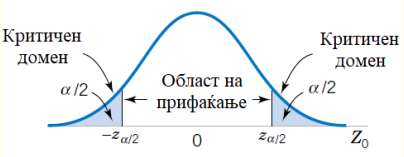
\includegraphics[width=0.7\textwidth]{image.png}
  \caption{}
  \label{fig:example_image}
\end{figure}


As mentioned earlier, we will not continue here with the explanation of the methods for determining the most powerful critical region for testing a hypothesis.  \\

But let us clarify why the critical region was chosen in this way. Why from the ends of the distribution?  \\

Let's see that the test statistic

\[  \frac{\bar{X}_n - \mu_0}{\sigma}\sqrt{n} \]

The test statistic, in a way, measures the difference between $\bar{X}_n$ (the estimated value of the mean in the given sample) and $\mu_0$ (the hypothesized value of the mean). The difference between them will be greater when $Z_0$ takes values further from 0.  \\

The alternative hypothesis is
\[
H_a: \mu \neq \mu_0,
\]
so we are interested in values on both sides of 0.\\


\textbf{Example 2:} Blood pressure in men aged \textbf{35} to \textbf{44} is known to have a normal
distribution with an expected value (mean) of \textbf{127} units with a
standard deviation of \textbf{7} units. During a systematic review of 70
randomly selected employees of a company, it was determined that
their average blood pressure is 125. At a significance level of $\alpha =0.05$, can it be concluded that the expected blood pressure of the
employees of that company deviates from the standards?\\


\subsubsection{One sided tests}

Next, we will consider one-sided tests:

\[
H_0: \mu = \mu_0, \quad H_a: \mu > \mu_0
\]
or
\[
H_0: \mu = \mu_0, \quad H_a: \mu < \mu_0
\]

The same test statistic $Z_0$ is used for testing, but now the critical region changes.  

In the first case, the critical region is
\[
C = (z_\alpha, +\infty),
\]

In the second case, it is
\[
C = (-\infty, -z_\alpha).
\]

Thus, $z_\alpha$ is the value from the standard normal distribution $N(0,1)$ for which
\[
\Phi(z_\alpha) = 1 - \alpha.
\]


\begin{figure}[h!]
  \centering
  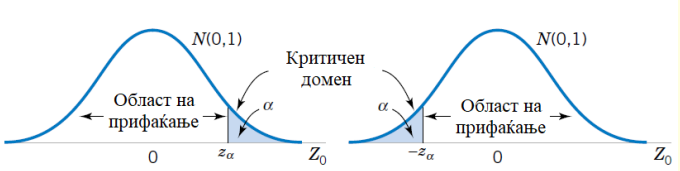
\includegraphics[width=1\textwidth]{image_2.png}
  \caption{}
  \label{fig:example_image}
\end{figure}


\subsubsection{Tests for the Mean of a Variable $X \sim N(\mu, \sigma^2)$
with Unknown $\sigma^2$ and Small Sample}

Let $X \sim N(\mu, \sigma^2)$, with $\sigma^2$ unknown and a small sample.  

Let the hypothesis be tested:

\[
H_0: \mu = \mu_0
\]
\[
H_a: \mu \neq \mu_0, \quad \text{or} \quad H_a: \mu > \mu_0, \quad \text{or} \quad H_a: \mu < \mu_0 \quad \text{(two-sided test)}.
\]

As before, we start from the estimator for $\mu$ obtained by the maximum likelihood method. That is,
\[
\hat{\mu} = \bar{X}_n,
\]
i.e., the sample mean.  

When the population variance $\sigma^2$ is unknown and the sample is small, then under the null hypothesis, the test statistic
\[
T_0 = \frac{\bar{X}_n - \mu_0}{S / \sqrt{n}} =\frac{\bar{X}_n - \mu_0}{S} \sqrt{n} 
\]
follows a $t$-distribution with $n-1$ degrees of freedom, where $S^2$ is the sample variance.\\

As in the previous case, the critical region depends on the alternative hypothesis.  

If we have a two-sided test, i.e., $H_a: \mu \neq \mu_0$, then the critical region is
\[
C = (-\infty, -t_{\alpha/2, n-1}) \cup (t_{\alpha/2, n-1}, +\infty),
\]
where $t_{\alpha/2, n-1}$ is obtained from the $t$-distribution table such that
\[
P\{T > t_{\alpha/2, n-1}\} = \frac{\alpha}{2}.
\]

If the alternative hypothesis is $H_a: \mu > \mu_0$, then the critical region is
\[
C = (t_{\alpha, n-1}, +\infty),
\]
where $t_{\alpha, n-1}$ is obtained from the $t$-distribution table such that
\[
P\{T > t_{\alpha, n-1}\} = \alpha.
\]

If the alternative hypothesis is $H_a: \mu < \mu_0$, then the critical region is
\[
C = (-\infty, -t_{\alpha, n-1}),
\]
where $t_{\alpha, n-1}$ is obtained from the $t$-distribution table such that
\[
P\{T > t_{\alpha, n-1}\} = \alpha.
\]

\begin{figure}[h]
  \centering
  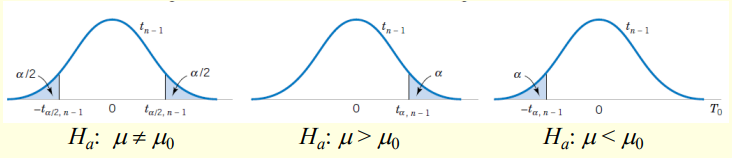
\includegraphics[width=1\textwidth]{image_3.png}
  \caption{}
  \label{fig:example_image}
\end{figure}


\textbf{Example 3:} It is known that the fuel consumption of Peugeot type cars has a
normal distribution with an expected value (mean) of \textbf{8} liters per \textbf{100}
kilometers. From the manufactured series, \textbf{17} cars were randomly
selected and an average consumption of \textbf{8.8} liters per \textbf{100} kilometers
with a standard deviation of \textbf{0.9} was obtained. With a significance
level of $\alpha = 0.05$, can it be argued that the car series has a higher than
predicted consumption?\\

\subsubsection{Tests for the Mean of a Variable $X \sim N(\mu, \sigma^2)$
with Unknown $\sigma^2$ and Large Sample}


Let $X \sim N(\mu, \sigma^2)$, with $\sigma^2$ unknown and a large sample.  

When a large sample is given ($n \ge 30$), replacing $\sigma$ with the sample standard deviation $S$ does not have a significant effect on the value of the $Z$ statistic. Therefore, we can approximate the $T$ statistic with the $Z$ statistic, i.e.,

\[
T_0 = \frac{\bar{X}_n - \mu_0}{S / \sqrt{n}} \approx Z_0,
\]

and use the corresponding $z$-tests.



\subsubsection{Tests for mean of feature with arbitrary distribution and large sample}

Often in practice, we cannot assume a normal distribution of the variable. However, when the sample is large ($n \ge 30$), then according to the central limit theorem, $Z$-statistics can be used to test hypotheses about the mean.  

If the variance of the variable is known, then the statistic used is
\[
Z_0 = \frac{\bar{X}_n - \mu_0}{\sigma / \sqrt{n}}.
\]

If the variance is unknown, then the statistic used is
\[
Z_0 = \frac{\bar{X}_n - \mu_0}{S / \sqrt{n}}.
\]

In both cases, when $H_0$ is true, $Z_0$ has an asymptotic standard normal distribution,
\[
Z_0 \sim N(0,1).
\]


\textbf{Example 4:} A drug factory produces antibiotics and the expected power (mean) of one of those antibiotics is $80\%$. A random sample of up to 100
capsules was tested and an average power of $79.7\%$ and a standard
deviation of $2\%$ was obtained. Are the antibiotics produced according
to the prescribed standards? Let $\alpha = 0.01$

\begin{figure}[h!]
  \centering
  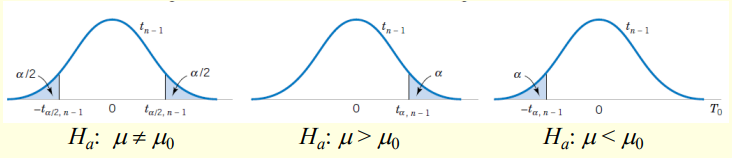
\includegraphics[width=0.8\textwidth]{image_3.png}
  \caption{Test statistics for mean}
  \label{}
  
\end{figure}


\textbf{p-test value}

One way to express the results of hypothesis testing is to state whether or not the null hypothesis is rejected for a predefined significance level $\alpha$.  

For example, we can say that 
\[
H_0: \mu = 50
\] 
is rejected at a significance level of 0.05. \\

However, this conclusion is often inadequate, as it does not inform the decision maker whether the calculated value of the test statistic is near the boundary of the critical region or far from it.\\

To avoid this, test results are often reported through the so-called
p-value of the test statistic.\\

\textbf{Definition 4.} The \textbf{p-value} represents the smallest level of
significance that would lead to the rejection of the null
hypothesis $H_0$ with the given data\\

If the significance level $\alpha$ is less than the obtained $p$-value, then the null hypothesis is accepted as true. Otherwise, it is rejected.  \\

The $p$-value carries more information about the strength of evidence against $H_0$, allowing the decision maker to draw a conclusion for any chosen significance level of the test.\\

\textbf{Example 5:} Let us consider the Example 4. A pharmaceutical factory produces antibiotics, and the expected potency of one of these antibiotics is 80\%. A random sample of \textbf{100} capsules was tested, and an average potency of 79.7\% and a standard deviation of 2\% were obtained. Are the produced antibiotics in accordance with the prescribed standards? Determine the p-value for this test. What can be concluded if $\alpha = 0.05$?


\subsection{Tests for statistical variance (and standard deviation) of feature with normal distribution}

\subsubsection{Test for the Variance of a Variable $X \sim N(\mu, \sigma^2)$ with $\mu$ and $\sigma$ unknown}

Let the variable $X$ have a normal distribution $N(\mu, \sigma^2)$, with both $\mu$ and $\sigma$ unknown.  

The null hypothesis is
\[
H_0: \sigma = \sigma_0
\]
versus one of the alternatives:
\[
H_a: \sigma \neq \sigma_0, \quad H_a: \sigma > \sigma_0, \quad \text{or} \quad H_a: \sigma < \sigma_0.
\]

For testing, the test statistic
\[
\chi_0^2 = \frac{(n-1) S^2}{\sigma_0^2}
\]
is used, which under the null hypothesis follows a chi-square distribution with $n-1$ degrees of freedom.\\

These are tests for the variance and standard deviation of a variable with a normal distribution.\\

As in the previous tests, the critical region depends on the alternative hypothesis.  

For $H_a: \sigma \neq \sigma_0$, the critical region is
\[
C = \left(0, \chi^2_{1-\alpha/2,\,n-1}\right) \cup \left(\chi^2_{\alpha/2,\,n-1}, +\infty \right).
\]

For $H_a: \sigma > \sigma_0$, the critical region is
\[
C = \left(\chi^2_{\alpha,\,n-1}, +\infty \right).
\]

For $H_a: \sigma < \sigma_0$, the critical region is
\[
C = \left(0, \chi^2_{1-\alpha,\,n-1} \right).
\]


\begin{figure}[h!]
  \centering
  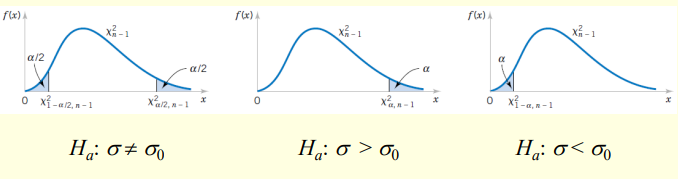
\includegraphics[width=0.8\textwidth]{image_5.png}
  \caption{}
  \label{}
\end{figure}

\textbf{Example 6:} Based on a random sample of size $n = 25$ for a normally distributed
feature $X$, a variance of 22 was obtained. With a significance level of 
$\alpha = 0.05$, can it be concluded that the variance of the feature is greater
than 15?

\section{TESTS FOR TWO FEATURES}

\subsection{Testing the \textbf{Equality of Variances} of two independent variables with Normal Distributions}  

Let $X$ and $Y$ be two statistical variables from two independent populations, with distributions 
\[
X \sim N(\mu_X, \sigma_X^2) \quad \text{and} \quad Y \sim N(\mu_Y, \sigma_Y^2),
\] 
where the parameters are unknown.  

Based on two independent random samples of size $n$ and $m$, respectively, we can test the null hypothesis
\[
H_0: \sigma_X^2 = \sigma_Y^2
\] 
versus one of its alternatives:
\[
H_a: \sigma_X^2 \neq \sigma_Y^2, \quad H_a: \sigma_X^2 > \sigma_Y^2, \quad \text{or} \quad H_a: \sigma_X^2 < \sigma_Y^2.
\]

Let 
\[
X = (X_1, \ldots, X_n)
\] 
be a random sample of feature $X$ measured in the first population, and 
\[
Y = (Y_1, \ldots, Y_m)
\] 
be a random sample of feature $Y$ measured in the second population.  \\

Let $S_X^2$ and $S_Y^2$ be the respective sample variances.\\

We have seen that the statistic
\[
F = \frac{S_X^2}{S_Y^2}
\]
has a Fisher $F_{n-1, m-1}$ distribution, with $n-1$ degrees of freedom in the numerator and $m-1$ degrees of freedom in the denominator.  \\

If the null hypothesis is true, the statistic will follow an $F_{n-1, m-1}$ distribution, and the critical regions will be defined based on this distribution.\\


As with the previous tests, the critical region depends on the alternative hypothesis.  

For $H_a: \sigma_X^2 \neq \sigma_Y^2$, the critical region is
\[
C = \left(0, f_{1-\alpha/2,\,n-1,\,m-1}\right) \cup \left(f_{\alpha/2,\,n-1,\,m-1}, +\infty \right).
\]

For $H_a: \sigma_X^2 > \sigma_Y^2$, the critical region is
\[
C = \left(f_{\alpha,\,n-1,\,m-1}, +\infty \right).
\]

For $H_a: \sigma_X^2 < \sigma_Y^2$, the critical region is
\[
C = \left(0, f_{1-\alpha,\,n-1,\,m-1} \right).
\]


\begin{figure}[h!]
  \centering
  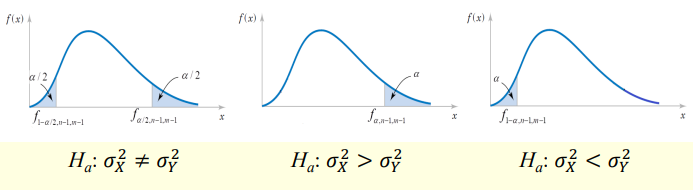
\includegraphics[width=0.8\textwidth]{image_6.png}
  \caption{}
  \label{fig:example_image}
\end{figure}

A problem with these tests can occur when determining the critical region, because the value must be obtained from the $F$-distribution.  \\

It is known that $F$-distribution tables exist only for a few (mainly smaller) values of $\alpha$.  \\

Therefore, determining the critical region when the alternative hypothesis is 
\[
H_a: \sigma_X^2 \neq \sigma_Y^2 \quad \text{or} \quad H_a: \sigma_X^2 < \sigma_Y^2
\] 
cannot be done directly.  

However, the following relationship can be used for the values of the $F$-distribution:
\[
f_{1-\alpha, m, n} = \frac{1}{f_{\alpha, n, m}}.
\]


\textbf{Example 7}  

One measure of the quality of blood glucose test strips is the consistency of test results on the same blood sample. Consistency is measured by the variances of readings in repeated testing. Suppose two types of strips, A and B, are being compared for their consistency. For testing, 16 strips of type A were taken and tested with drops of blood from one test tube (previously mixed well), and a variance of  $s_A^2 = 2.09$ was obtained.  

Also, 21 strips of type B were tested with drops of blood from the same test tube, and a variance of  $s_B^2 = 1.1$ was obtained. It is assumed that both samples are taken from normally distributed populations. At a significance level of 0.1, test whether the consistency of the two types of strips is equal.


\subsection{Testing the \textbf{Equality of Means} of Two Independent Statistical Features (Two Populations)}  

Let 
\[
X = (X_1, \ldots, X_n)
\] 
be a random sample of feature $X$ measured on one population, and 
\[
Y = (Y_1, \ldots, Y_m)
\] 
be a random sample of feature $Y$ measured on another population, with means $\mu_X$ and $\mu_Y$ respectively, which are unknown. \\ 

We want to test whether $\mu_X$ and $\mu_Y$ are equal.  

The null hypothesis is
\[
H_0: \mu_X = \mu_Y
\] 
versus one of the alternatives:
\[
H_a: \mu_X \neq \mu_Y, \quad H_a: \mu_X > \mu_Y, \quad \text{or} \quad H_a: \mu_X < \mu_Y.
\]  

We distinguish two cases:  
\begin{itemize}
  \item  [1.] Small samples for features with normal distributions, with known or unknown standard deviations.  
  \item [2.] Large samples for features with unknown standard deviations.\\
\end{itemize}


\subsubsection{Test for $X \sim N(\mu_X, \sigma_X^2), \quad Y \sim N(\mu_Y, \sigma_Y^2)$, with known variances $\sigma_X^2$ and $\sigma_Y^2$, and sample sizes $n, m < 30$.  }

In this case, the following test statistic is used, which has a standard normal distribution $N(0,1)$.  

When the null hypothesis 
\[
H_0: \mu_X = \mu_Y
\] 
is true, the test statistic takes the form:
\[
Z_0 = \frac{\bar{X} - \bar{Y} - (\mu_X - \mu_Y)}{\sqrt{\sigma_X^2 / n + \sigma_Y^2 / m}} 
= \frac{\bar{X} - \bar{Y}}{\sqrt{\sigma_X^2 / n + \sigma_Y^2 / m}}.
\]

The critical region depends on the alternative hypothesis and is obtained from the standard normal distribution table.  \\

If we assume that the variances are equal, i.e., 
\[
\sigma_X^2 = \sigma_Y^2 = \sigma^2,
\] 
we estimate the common variance with the pooled variance statistic
\[
S_p^2 = \frac{(n-1)S_X^2 + (m-1)S_Y^2}{n + m - 2},
\] 
and then the test statistic is
\[
T_0 = \frac{\bar{X} - \bar{Y}}{S_p \sqrt{1/n + 1/m}}.
\]  

When the null hypothesis is true, $T_0$ has a $t$-distribution with $n + m - 2$ degrees of freedom. Using this fact, we determine the appropriate critical regions for the $t$-test.\\


The assumption for this test is that the variances of the two variables are equal, i.e.,
\[
\sigma_X^2 = \sigma_Y^2 = \sigma^2.
\]

However, since the variances are unknown, the question arises: how do we know if they are equal?  \\

In such a case, a test for equality of variances is conducted first.  \\

If this test passes, then the test of equality of means can be performed. Otherwise, the test of equality of means may not give relevant results.  \\

\textbf{Note:} Since the $t$-distribution table contains values only for degrees of freedom $\le 30$, if $n + m - 2 > 30$, when determining the critical region we can use
\[
t_{\alpha, n+m-2} \approx z_\alpha,
\]
i.e., in this case, the critical values can be read from the standard normal $N(0,1)$ table.\\


\textbf{Example 8}

By measuring the time needed to manufacture chips using one technological
process, the following data were obtained: 53, 119, 104, 137, 119, 117, 104,
73, 53, 69, 119. Thirteen measurements were also taken of the time needed to
manufacture the same chip using another technological process. For this
second process, the observed times have a mean value of 56 and a variance
of 640.3. We assume that the manufacturing times are normally distributed.
At a 5\% significance level, test the hypothesis that the second process is
faster than the first\\


\subsubsection{Test for Arbitrary Distribution of $X$ and $Y$, $m, n \ge 30$}  

When dealing with large samples, the $Z$-statistic is used to test these hypotheses. Its form depends on whether the feature variances are known or unknown.  \\

If the variances of the features are known, the test statistic is
\[
Z_0 = \frac{\bar{X} - \bar{Y}}{\sqrt{\sigma_X^2 / n + \sigma_Y^2 / m}}.
\]

If the variances of the features are unknown, the test statistic is
\[
Z_0 = \frac{\bar{X} - \bar{Y}}{\sqrt{S_X^2 / n + S_Y^2 / m}}.
\]

In both cases, when the null hypothesis is true, $Z_0$ has an approximate standard normal distribution, $N(0,1)$, so the critical regions for $z$-values are used for testing.  \\

The critical region depends only on the alternative hypothesis.  \\

All the tests we have considered so far are tests in which the null hypothesis is simple and the alternative hypothesis is complex.  \\

It is important to note that if the alternative hypothesis remains the same and the null hypothesis becomes complex, the critical region does not change.\\  

It is also important to be aware that the sets of parameter values in the null and alternative hypotheses must be disjoint, so that rejecting one hypothesis implies accepting the other. \\

\textbf{Critical domain:}
If a mean value test is conducted, then we have the following
cases.


\begin{figure}[h!]
  \centering
  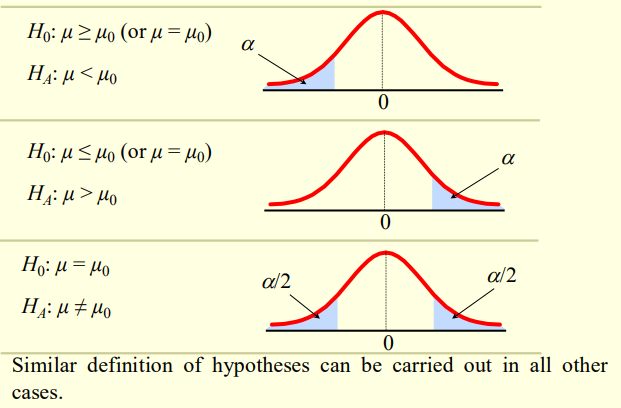
\includegraphics[width=0.8\textwidth]{image_7.png}
  \caption{}
  \label{fig:example_image}
\end{figure}


\null
\newpage
\textbf{Example 9}
Research has been done on the average salary of IT engineers. A
sample of 50 IT engineers was taken and it was found that their
average salary is $62570$ denars with a standard deviation of $7500$
denars. With a significance level of 0.05, test the hypothesis that the
average salary is at least $61500$ denars against the alternative that it is
less than $61500$ denars.


\tableofcontents
\end{document}